\subsection{Waveforms}

\begin{figure} [H]
    \centering
    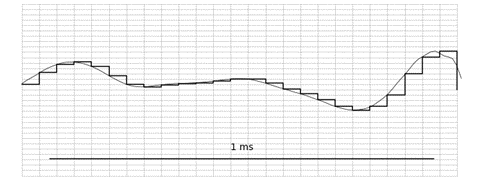
\includegraphics[width=0.75\linewidth]{images/audiorep/waveform.png}
    \caption{Each value within the waveform is sampled at a consistent rate and precisely quantized, enabling accurate digital representation of the audio. }
    \label{fig:waveform}
\end{figure}

Ever wonder what that squiggly line on your music player represents? That's a waveform, a digital picture of sound! Picture sound waves like ripples in a pond: a microphone captures these air pressure changes and turns them into an electrical signal. This signal is then chopped up and packaged into bite-sized pieces (sampled) and given labels (quantized) before ending up as the waveform you see. Don't worry about the fancy terms just yet, remember continuous sound gets turned into tiny, numbered points to play on your computer.

There's just one channel (mono) if it's like a single line, but two channels (stereo) if it's like two squiggly lines stacked together. That's all you need to know for now!

Imagine you're trying to recreate a picture by tracing its outlines with dots. The more dots you use, the smoother and more accurate your picture will be. That's the essence of sample rate in audio recordings like speech.

There are some important definitions related to this representation: 
\begin{itemize}
    \item \textbf{Sample rate:} How often we "sample" or capture sound waves per second, measured in Hertz (Hz). Higher rates capture more detail, especially high-pitched sounds.
    \item \textbf{Nyquist frequency:} The highest frequency a sample rate can accurately represent. It's half the sample rate. Think of it as the "sound ceiling" – anything higher gets distorted.
    \item \textbf{Downsampling:} Reducing the sample rate, sacrificing detail for efficiency. Like using fewer dots for your picture, it can save processing power while still conveying the main idea.
\end{itemize}
While downsampling can be helpful for faster model training, it's important to choose wisely. Dropping the rate too much can "throw away" important high-frequency sounds, impacting the clarity and quality of the enhanced speech.
